\section{Offset, Amplitude, Frequenz und Phase eines Pendels}

\subsection{Arbeitsgrundlagen}

Die ged\"ampfte Schwingung eines Pendels kann mit der Formel
\begin{equation}
    y = A \cdot e^{-\Gamma \cdot t} \cdot \sin(2\pi f t - \delta) + y_0
    \hspace{5mm} \textrm{wobei} \hspace{5mm}
    \begin{tabular}{ll}
        $A$:        & Amplitude \\
        $\Gamma$:   & Abklingkonstante \\
        $f$:        & Frequenz in Hz \\
        $\delta$:   & Phase \\
        $y_0$:      & Offset \\
    \end{tabular}
    \label{eq:gedaempfte-schwingung}
\end{equation}
beschrieben werden.


\subsection{Durchf\"uhrung}

\subsubsection*{Versuchsanordnung}

Die ged\"ampfte Schwingung eines Pendels wurde mittels Ultraschallsensor vermessen. Die Zeitabh\"angige
Positionsdaten sind in der Tabelle \ref{tab:pendel} aufgezeichnet.


\subsubsection*{Messergebnisse}

\begin{center}
    \begin{threeparttable}
        \caption{Gemessene Gr\"ossen}
        \begin{tabular}{*{12}{c}}
            \toprule
            $t(s)$  &  $y(m)$   &  $t(s)$   &  $y(m)$   &  $t(s)$  &  $y(m)$    &  $t(s)$   & $y(m)$    &  $t(s)$   &  $y(m)$   &  $t(m)$   &  $y(m)$ \\
            \midrule
            0.5     & -0.352    & 8.0       & 0.630     & 15.5     & -0.572     & 23.0      & 0.409    & 30.5       & -0.018    & 38.0      & 0.072   \\
            1.0     & -0.204    & 8.5       & 0.538     & 16.0     & -0.439     & 23.5      & 0.411    & 31.0       & -0.041    & 38.5      & 0.006   \\
            1.5     & 0.124     & 9.0       & 0.434     & 16.5     & -0.362     & 24.0      & 0.472    & 31.5       & -0.147    & 39.0      & 0.136   \\
            2.0     & 0.255     & 9.5       & 0.323     & 17.0     & -0.394     & 24.5      & 0.381    & 32.0       & -0.095    & 39.5      & 0.180   \\
            2.5     & 0.302     & 10        & 0.185     & 17.5     & -0.211     & 25.0      & 0.448    & 32.5       & -0.144    & 40.0      & 0.110   \\
            3.0     & 0.516     & 10.5      & 0.068     & 18.0     & -0.292     & 25.5      & 0.379    & 33.0       & -0.232    & 40.5      & 0.087   \\
            3.5     & 0.754     & 11.0      & -0.073    & 18.5     & -0.122     & 26.0      & 0.340    & 33.5       & -0.162    & 41.0      & 0.225   \\
            4.0     & 0.819     & 11.5      & -0.204    & 19.0     & -0.008     & 26.5      & 0.203    & 34.0       & -0.112    & 41.5      & 0.113   \\
            4.5     & 0.866     & 12.0      & -0.248    & 19.5     & 0.084      & 27.0      & 0.184    & 34.5       & -0.171    & 42.0      & 0.184   \\
            5.0     & 0.916     & 12.5      & -0.353    & 20.0     & 0.126      & 27.5      & 0.111    & 35.0       & -0.086    & 42.5      & 0.167   \\
            5.5     & 1.014     & 13.0      & -0.392    & 20.5     & 0.192      & 28.0      & 0.089    & 35.5       & -0.130    & 43.0      & 0.198   \\
            6.0     & 0.942     & 13.5      & -0.576    & 21.0     & 0.200      & 28.5      & 0.094    & 36.0       & -0.075    & 43.5      & 0.212   \\
            6.5     & 0.931     & 14.0      & -0.543    & 21.5     & 0.216      & 29.0      & 0.106    & 36.5       & -0.098    & 44.0      & 0.142   \\
            7.0     & 0.858     & 14.5      & -0.468    & 22.0     & 0.400      & 29.5      & -0.003   & 37.0       & 0.056     & 44.5      & 0.128   \\
            7.5     & 0.678     & 15.0      & -0.496    & 22.5     & 0.329      & 30.0      & -0.013   & 37.5       & 0.056     & 45.0      & 0.138   \\
            \bottomrule
        \end{tabular}
        \begin{tablenotes}
            \small
            \item \textbf{Hinweis:} Daten wurden vom Auftragsdokument kopiert.
        \end{tablenotes}
        \label{tab:pendel}
    \end{threeparttable}
\end{center}

Die Amplitude $A$, Abklingkonstante $\Gamma$, Frequenz $f$, Phase $\delta$ und Offset $y_0$ sollen
ermittelt werden.


\subsubsection*{QtiPlot}

\begin{figure}[H]
    \center
    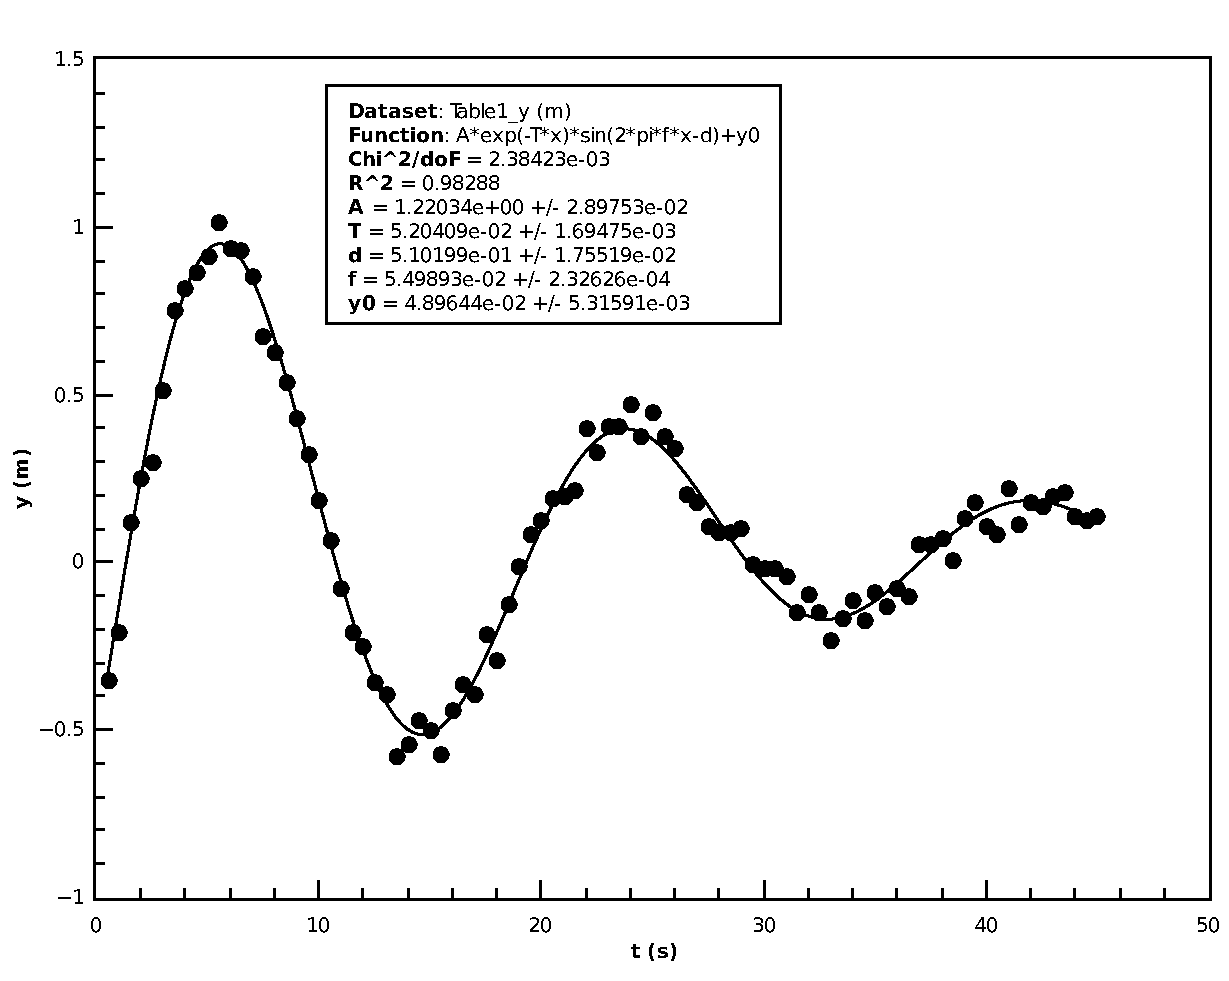
\includegraphics[width=.85\textwidth]{qtiplot/pendel}
    \caption{Nicht-lineare Regression zur Bestimmung von $A$, $\Gamma$, $f$, $\delta$ und $y0$}
    \label{fig:pendel}
\end{figure}

Die Formel \ref{eq:gedaempfte-schwingung} wird in QtiPlot als Fit-Funktion eingegeben. Die gesuchten
Parameter k\"onnen mittels nicht-linearer Regression ermittelt werden. Aufgrund der nicht-linearen Art
der Formel m\"ussen vor dem Fitten gute Startwerte von Hand eingestellt werden. Dazu wird der Checkbox
``Preview'' eingeschalten und mit den Parametern gespielt, bis die Kurve ungef\"ar passt.


\subsection{Resultate und Diskussion}

Von der Figur \ref{fig:pendel} k\"onnen die gesuchten Parameter abgelesen werden. Diese sind:
\begin{center}
    \begin{tabular}{ll}
        Amplitude $A$:              &  $(1.22 \pm 0.03)$         \\
        Abklingkonstante $\Gamma$:  &  $(52.0 \pm 1.69)\num{e-3}$ \\
        Phase $\delta$:             &  $(510  \pm 17.6)\num{e-3}$ \\
        Frequenz $f$:               &  $(55.0 \pm 23.3)\num{e-3}$ \\
        Offset $y_0$:               &  $(49.0 \pm 5.32)\num{e-3}$ \\
    \end{tabular}
\end{center}

